\subsection{Layout and Formats}

\begin{frame}{Frame size and chroma sub-sampling}
  \begin{itemize}
  \item Digital pictures easily take up a lot of space (more so for videos)
  \item The minimal size for a picture depends on:
    \begin{itemize}
    \item Dimensions (\(width\) and \(height\))
    \item Number of bits per pixel (\(bpp\)): color (and alpha) depth and dead bits
    \item Roughly: \(width \times height \times bpp \div 8~bytes\)
    \item For 12 Mpixels with 16 Mcolors and alpha: \(4000 \times 3000 \times 32 \div 8 = 45.8 MiB\)
    \end{itemize}
  \item The human visual system has specificities:
    \begin{itemize}
    \item High sensitivity to \textbf{luminosity} (luminance)
    \item Low sensitivity to \textbf{colors} (chrominance)
    \end{itemize}
  \item The YUV color model offers the relevant channel separation
  \item Sub-sampling can be applied to the chrominance channel\\
  \textit{less data (and precision) on colors to reduce size}
  \end{itemize}
\end{frame}

\begin{frame}{Frame size and chroma sub-sampling}
  \begin{itemize}
  \item Chrominance samples are used for multiple luminance samples
  \item With specific vertical and horizontal ratios (usually integer)
  \item Usually summarized using a three-part ratio: \(J:a:b\)
  \end{itemize}

  \begin{center}
  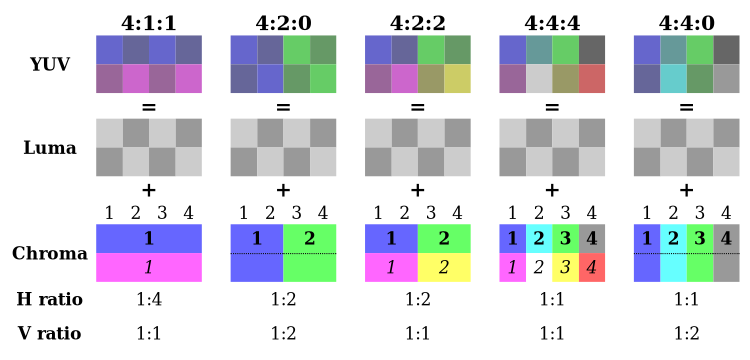
\includegraphics[width=0.55\textwidth]{slides/graphics-theory-layout-formats/yuv-sub-sampling.pdf}

  YUV 4:2:0 usual example:
  {\small
  \begin{equation*}
  \begin{gathered}
  bpp_Y = 8,~bpp_U = bpp_V = 8 \div 2 \div 2 = 2 \\
  \Rightarrow~ bpp = bpp_Y + bpp_U + bpp_V = 12~bits/pixel
  \end{gathered}
  \end{equation*}
  }
  \end{center}
\end{frame}

\begin{frame}{Pixel data distribution in memory}
  \begin{itemize}
  \item Pixel data can be \textbf{distributed} in different ways in memory
  \item Different ways to aggregate color components in \textbf{data planes} (memory chunks):
    \begin{itemize}
    \item \textbf{Packed}: Components are stored in the same data plane in memory
    \item \textbf{Semi-planar} (YUV): Luma and chroma are stored in distinct data planes
    \item \textbf{Planar}: Each component has its own data plane in memory
    \end{itemize}
  \item When multiple color components are grouped, \textbf{bit order} must be specified:
    \begin{itemize}
    \item Which component comes first in memory?
    \item Affected by endianness when read by hardware!
    \end{itemize}
  \item \textbf{Scan order} must also be specified:
    \begin{itemize}
    \item How to calculate the address for position \((x,y)\) and back?
    \item Raster order (most common) specifies: row-major, left-to-right, top-to-bottom
    \end{itemize}
  \end{itemize}
  \begin{center}
  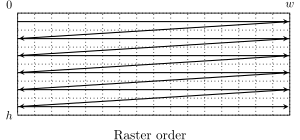
\includegraphics[height=6em]{slides/graphics-theory-layout-formats/raster-order.pdf}
  \end{center}
\end{frame}

\begin{frame}[fragile]{Pixel formats, FourCC codes}
  \begin{itemize}
  \item Many meta-data elements are needed to fully describe how a picture is coded
    \begin{itemize}
    \item Some describe \textbf{picture-level attributes} (e.g. dimensions)
    \item Some describe \textbf{pixel-level attributes} (e.g. colorspace, bpp)
    \end{itemize}
  \item Pixel-level attributes are grouped as a \textbf{pixel format} that defines:
    \begin{itemize}
    \item Color model in use
    \item Number of bits per channel and per pixel (bpp)
    \item Bit attribution and byte order
    \item Per-channel sub-sampling ratios
    \item Pixel data planes distribution in memory
    \end{itemize}
  \item Often represented as a 4-character code called \textbf{FourCC}\\
  \item Not really standardized and implementation-specific:\\
    \textit{DRM in Linux uses \code{XR24} for \ksym{DRM_FORMAT_XRGB8888}}.\\
  \textit{Not really standardized but widely used in various forms}
  \item Scan order is specified separately with a \textbf{modifier}\\
    \textit{Assumed to be raster order if unspecified}
  \end{itemize}
\end{frame}

\begin{frame}{Level of detail of quantized pictures}
  Depends on a number of factors, including:
  \begin{itemize}
  \item Spatial density (pixel resolution)
  \item Quantized dimensions (picture width and height)
  \item Colorspace limits (chromaticity diagram)
  \item Color depth (number of bits per pixel)
  \item Color resolution and range trade-off
  \end{itemize}~

  Generally speaking:
  \begin{itemize}
  \item Many factors are involved
  \item The major bottleneck is not always obvious
  \item Implementation choices do matter
  \end{itemize}
\end{frame}
